\renewcommand*\chappic{img/intro.pdf}
\renewcommand*\chapquote{}
\renewcommand*\chapquotesrc{}
\chapter{Introduction}
\label{ch:intro}
%
Hash functions are used as cryptographic primitives in many applications and protocols.
They take an arbitrary input message and provide a hash value. Input message and hash value
are considered as byte strings in a particular encoding.
The hash value is of fixed length and satisfies several properties which make it useful
in a variety of applications.

In this thesis we will consider the hash algorithms MD4 and SHA-256 and represent
differential characteristics of hash collisions as SAT problem. If and only if
satisfiability is given, the particular differential state is achievable
using two different inputs leading to the same output. As far as SAT solvers
return an actual model satisfying that state, we get an actual hash collision
which can be verified and visualized.
If the internal state of the hash algorithm is too large, the attack can be
computationally simplified by modelling only a subset of steps of the hash algorithm
or changing the modelled differential path.

Based on experience with these kind of problems with previous non-SAT-based tools
we aim to apply best practices to a satisfiability setting.
We will discuss which SAT techniques lead to best performance characteristics
for our MD4 and SHA-256 testcases.

\newpage  % FIX manual pagebreak
\section{Cryptanalysis preliminaries}
\label{sec:intro-crypt-prelim}
%
\index{Hash value}
\index{Preimage}
\index{Hash function}
\begin{defi}[Hash function]
  A \emph{hash function} is a mapping $h: X \to Y$ with $X = \left\{0,1\right\}^*$ and
  $Y = \left\{0,1\right\}^n$ for some fixed $n \in {\mathbb{N}}_{\geq 1}$.
  \begin{itemize}[noitemsep,topsep=0pt]
    \item Let $x \in X$, then $h(x)$ is called \emph{hash value of $x$}.
    \item Let $h(x) = y \in Y$, then $x$ is called \emph{preimage of $y$}.
  \end{itemize}
\end{defi}

One example showing the use of hash functions as primitives are JSON Web Tokens (JWT)
specified in RFC~7519~\cite{rfc7519}. Section~8 defines implementation requirements
and refers to RFC~7518~\cite{rfc7518}, which specifies cryptographic algorithms to
be implemented. \enquote{HMAC SHA-256} (besides \enquote{none}) is the only signature
and MAC algorithm required to be implemented.
SHA-256 as hash algorithm is used as cryptographic primitive in this configuration.

A hash function has to satisfy the following security requirements:

\index{Preimage resistance}
\begin{defi}[Preimage resistance]
  Given $y \in Y$,
  a hash function $h$ is \emph{preimage resistant} iff it is computationally infeasible
  to find $x \in X$ such that $h(x) = y$.
\end{defi}

\index{Second-preimage resistance}
\begin{defi}[Second-preimage resistance]
  Given $x \in X$,
  a hash function $h$ is \emph{second-preimage resistant} iff it is computationally infeasible
  to find $x_2 \in X$ with $x \neq x_2$ such that $h(x) = h(x_2)$.
  $x_2$ is called \emph{second preimage}.
\end{defi}

\index{Collision resistance}
\begin{defi}[Collision resistance]
  A hash function $h$ is \emph{collision resistant} iff it is computationally infeasible to
  find any two $x \in X$ and $x_2 \in X$ with $x \neq x_2$ such that $h(x) = h(x_2)$.
\end{defi}

As far as hash functions accept input strings of arbitrary length, but return a fixed
size output string, existence of collisions is unavoidable~\cite{schlaffer}.
However, good hash functions make it very difficult to find collisions or preimages.

The considered hash functions apply padding to their input to normalize their
input size to a multiple of its block size. The round function follows afterwards.
In the following, we always consider input of block size instead of the original
input message as bytestring.
Padding is negligible, because once we have two colliding blocks,
the collision will be reflected in the output in these single-pipe Merkle-Darmg\aa rd designs.
This results in a length extension attack, making input padding negligible for cryptanalysis.

\section{Cryptanalysis of Hash Functions}
\label{sec:intro-cryptanalysis}
%
In August 2004, Wang et al. published results at Crypto'04~\cite{wang2004} which revealed
that MD4, MD5, HAVAL-128 and RIPEMD can be broken practically using differential cryptanalysis.
Their work is based on preliminary work by Hans Dobbertin~\cite{Dobbertin1998}.
On an IBM~P690 machine, an MD5 collision can be computed in about one hour using this approach.
Collisions for HAVAL-128, MD4 and RIPEMD were found as well. Patrick Stach's \texttt{md4coll.c}
program~\cite{md4coll} implements Wang's approach and can find MD4 collisions in few seconds
on my Thinkpad~x220 setup specified in \hyperref[app:setup]{Appendix~\ref{app:setup}}.

Let $n$ denote the digest size, i.e. the size of the hash value $h(x)$ in bits.
Due to the birthday paradox, a collision attack has a generic complexity of $2^{n/2}$
whereas preimage and second preimage attacks have generic complexities of $2^n$.
In other words it is computationally easier to find any two colliding hash values
than the preimage or second preimage for a given hash value.

Following results by Wang et al., differential cryptanalysis was shown as
powerful tool for cryptanalysis of hash algorithms. This thesis applies those
ideas to satisfiability approaches.

\begin{table}[bt]
  \begin{center}
    \begin{tabular}{cccc}
      \hline \hline
      \multicolumn{4}{c}{Message 1} \\
      \hline
      4d7a9c83 & \textbf{d6cb927a} & \textbf{29d5a578} & 57a7a5ee \\
      de748a3c & dcc366b3 & b683a020 & 3b2a5d9f \\
      c69d71b3 & f9e99198 & d79f805e & a63bb2e8 \\
      \textbf{45dc8e31} & 97e31fe5 & 2794bf08 & b9e8c3e9 \\
      \hline
      \multicolumn{4}{c}{Message 2} \\
      \hline
      4d7a9c83 & \textbf{56cb927a} & \textbf{b9d5a578} & 57a7a5ee \\
      de748a3c & dcc366b3 & b683a020 & 3b2a5d9f \\
      c69d71b3 & f9e99198 & d79f805e & a63bb2e8 \\
      \textbf{45dd8e31} & 97e31fe5 & 2794bf08 & b9e8c3e9 \\
      \hline
      \multicolumn{4}{c}{Hash value of Message 1 and Message 2} \\
      \hline
      5f5c1a0d & 71b36046 & 1b5435da & 9b0d807a \\
      \hline \hline
    \end{tabular}
    \caption[Hexadecimal values of one MD4 collisions given in paper~\cite{wang2004}]{
      One of two MD4 hash collisions provided in~\cite{wang2004}.
      Values are given in hexadecimal, message words are enumerated from
      left to right, top to bottom. Differences are highlighted in
      bold for illustration purposes. For comparison the first bits
      of Message 1 are \texttt{11000001\dots} and the last bits are
      \texttt{\dots10011101}.
      A message represents one block of 512~bits.
      %The hash value consists of 128~bits.
    }
    \label{tab:wang-md4-collision1}
  \end{center}
\end{table}

\newpage
\section{Differential cryptanalysis}
\label{sec:intro-diff-cryptanalysis}
%
\index{Hash collision}
\begin{defi}[Hash collision]
  Given a hash function $h$,
  a hash collision is a pair $(x, x_2)$ with $x \neq x_2$ such that
  $h(x) = h(x_2)$.
\end{defi}

Differential cryptanalysis is based on the idea to consider two execution states
of hash algorithms for slightly different input messages. We trace those difference
to learn about the propagation of message differences.

Hash algorithms consume input values as blocks of bits.
As far as the length of the input must not conform to the block size,
padding is applied. Now consider such a block of input values
and another copy of it. We use those two blocks as inputs for two
hash algorithm implementations, but provide slight modifications in few bits.
MD4 has 48 round function applications in 3 rounds.
Differential cryptanalysis considers the difference in the evaluation
state between the two instances (compare with Figure~\ref{tab:collision-attack}).

Visualizing those differences helps the cryptanalyst to find modifications yielding
a small number of differences in the evaluation state.
The cryptanalyst consecutively modifies the input values to eventually
receive a collision in the output value.
If the number of differences in the evaluation state is small,
this trail is expected to result in a hash collision with higher probability.

\begin{figure}[pbt]
  \begin{center}
    \fbox{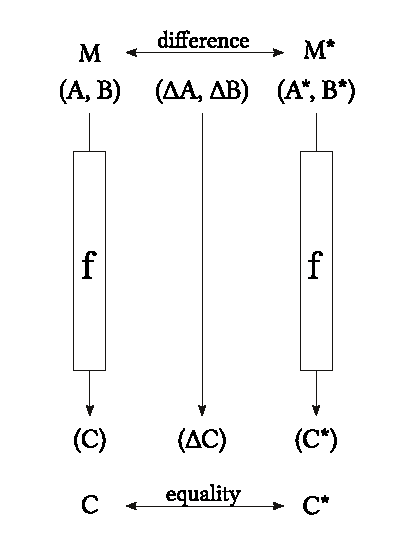
\includegraphics[width=0.55\textwidth]{img/diff_cryptanalysis.pdf}}
    \caption[Typical attack setting for a collision attack]{
      Typical attack setting for a collision attack:
      Hash function $f$ is applied to two inputs $M$ and $M^*$ which differ
      by some predefined bits. $\triangle M$ describes the difference between
      these values. A hash collision is given if and only if output values
      $C$ and $C^*$ show the same value. In differential cryptanalysis we observe
      the differences between two instances applying function $f$
      to inputs $M$ and $M^*$.
    }
    \label{tab:collision-attack}
  \end{center}
\end{figure}

\section{Satisfiability}
\label{sec:intro-sat}
%
\index{Boolean function}
\begin{defi}
  A \emph{Boolean function} is a mapping $h: X \to Y$ with $X = \left\{0,1\right\}^n$
  for $n \in \mathbb N_{\geq 1}$ and $Y = \left\{0,1\right\}$.
\end{defi}

The following definition gives three basic Boolean functions:

\index{AND (Boolean function)}
\index{OR (Boolean function)}
\index{NOT (Boolean function)}
\begin{defi}
  Let \boolf{AND}, \boolf{OR} and \boolf{NOT} be three Boolean functions.
  \begin{itemize}[noitemsep,topsep=0pt]
    \item
      \boolf{AND} maps $X = \left\{0,1\right\}^2$
      to $1$ if all values of $X$ are $1$.
    \item
      \boolf{OR} maps $X = \left\{0,1\right\}^2$
      to $1$ if any value of $X$ is $1$.
    \item
      \boolf{NOT} maps $X = \left\{0,1\right\}^1$
      to $1$ if the single value of $X$ is $0$.
  \end{itemize}
  All functions return $0$ in the other case.
\end{defi}

\index{Truth table}
\begin{defi}
  A \emph{truth table} unambiguously defines a Boolean function
  by enlisting the evaluated truth value for all possible sets of
  inputs.

  Table~\ref{tab:andornot-truthtables} shows truth tables for
  \boolf{AND}, \boolf{OR} and \boolf{NOT}.
\end{defi}

\begin{table}[pt]
  \centering
  \subfloat[\boolf{AND}]{%
    \begin{tabular}{cc|c}
      $v_1$ & $v_2$ & $f(v_1, v_2)$ \\
     \hline
      $1$ & $1$ & $1$ \\
      $1$ & $0$ & $0$ \\
      $0$ & $1$ & $0$ \\
      $0$ & $0$ & $0$
    \end{tabular}
  }
  ~
  \subfloat[\boolf{OR}]{%
    \begin{tabular}{cc|c}
      $v_1$ & $v_2$ & $f(v_1, v_2)$ \\
     \hline
      $1$ & $1$ & $1$ \\
      $1$ & $0$ & $1$ \\
      $0$ & $1$ & $1$ \\
      $0$ & $0$ & $0$
    \end{tabular}
  }
  ~
  \raisebox{13.6pt}{%
    \subfloat[\boolf{NOT}]{%
      \begin{tabular}{c|c}
        $v$ & $f(v)$ \\
       \hline
        $1$ & $0$ \\
        $0$ & $1$
      \end{tabular}
    }%
  }%
  \caption{Truth tables for \boolf{AND}, \boolf{OR} and \boolf{NOT}}
  \label{tab:andornot-truthtables}
\end{table}

Boolean functions have an important property which is characterized
in the following definition:

\index{Satisfiability}
\index{Assignment}
\index{Model}
\begin{defi}
  A Boolean function $f$ is \emph{satisfiable} iff there exists at least one
  input $x \in X$ such that $f(x) = 1$.
  Every input $x \in X$ satisfying this property is called \emph{model}.
  Every element of $X$ is called \emph{assignment}.
\end{defi}

The generic complexity of SAT determination is given by $2^n$ for $n$ Boolean variables.
%This is closely related to the \cP $\overset{?}{\neq}$ \cNP question.
The corresponding tool to determine satisfiability is defined as follows:

\index{SAT solver}
\begin{defi}
  A \emph{SAT solver} is a tool to determine satisfiability of a Boolean function.
  If satisfiability is given, it returns some model.
\end{defi}

SAT research is heavily concerned with finding good heuristics to find some model
for a given SAT problem as fast as possible. Biyearly
\href{http://satcompetition.org/}{SAT competitions} take place to challenge
SAT solvers in a set of benchmarks. The committee evaluates the most successful
SAT solvers solving the most problems within a given time frame.

\section{Satisfiability of hash algorithm states}
\label{sec:intro-algo-sat}
%
We discussed Boolean functions and satisfiability. At the same time we looked
at basic properties of hash algorithms. But the question remains how we can
link those areas together? This section is dedicated to this question.

\index{Algorithm}
\index{I/O Algorithm}
\begin{defi}
  An \emph{algorithm} is a step-wise set of instructions to solve a problem.
  An \emph{I/O algorithm} transforms given input values to output values.
\end{defi}

Hash algorithms are one example of I/O algorithms.

I/O algorithms can be implemented as a sequence of instructions for computers.
At the same time I/O algorithms can be represented as combination of Boolean
functions. This claim is backed in more detail in Section~\ref{sec:sat-dimacs}
with Theorem~\ref{thm:all-cnf}. It follows immediately that we can represent
I/O algorithms such as hash algorithms entirely as Boolean function.

\begin{theorem}
  Every algorithm can be represented as Boolean function.
\end{theorem}

\index{Least significant bit}
\index{Most significant bit}
We consider 2bit addition as small example. Let $a_{i}$ be the first argument
where $i$ denotes the binary position. If $i=0$, the \emph{least significant bit}
(LSB) is considered. If $i=1$, the \emph{most significant bit} (MSB) is considered.

Let $b_{i}$ be the second argument and $s_{i}$ be the output value.
Furthermore $c_{i}$ is the carry bit, where $c_1$ is left out, because
it is not used in 2bit addition. This model of 2bit addition as Boolean
function can be seen in Figure~\ref{fig:intro-2bit-addition}.

\begin{figure}
  \begin{center}
    \begin{tabular}{lrcc}
      1st arg: &   & $a_{1}$ & $a_{0}$ \\
      2nd arg: & + & $b_{1}$ & $b_{0}$ \\
    \hline
      carry:   &   &         & $c_0$ \\
      sum:     & = & $s_{1}$ & $s_0$
    \end{tabular}
    \hspace{10pt}~$\leadsto$\hspace{10pt}%
    \begin{minipage}{50pt}%
      \begin{flalign*}
        s_0 &= \boolf{XOR}(a_0, b_0) &\\
        c_0 &= a_0 \land b_0 &\\
        s_1 &= \boolf{XOR}(a_0, b_0, c_0) &
      \end{flalign*}
    \end{minipage}
  \end{center}
  \caption{Modelling 2bit addition (left) as Boolean function (right)}
  \label{fig:intro-2bit-addition}
\end{figure}

\section{Thesis Outline}
\label{sec:intro-outline}
%
This thesis is organized as follows:

\begin{description}
\item[In Chapter~\ref{ch:intro}] we discussed the basic properties and fundamentals
of the tools in discussion including hash functions and SAT solvers.

\item[In Chapter~\ref{ch:dc}] we introduce the MD4 and SHA-256 hash functions and
discuss possible approaches in differential cryptanalysis.

\item[In Chapter~\ref{ch:sat}] we discuss SAT solving and potential
approaches to speed up SAT solvers for cryptographic problems.

\item[In Chapter~\ref{ch:results}] we show results of our work
and discuss its implications.

\item[In Chapter~\ref{ch:summary}] we suggest future work based on our results.
\end{description}
